\documentclass{standalone}
\usepackage{tikz}
\usetikzlibrary{patterns}

\tikzset{
  svgfrag/.style 2 args={
    execute at begin scope={\special{dvisvgm:raw <g class="fragment #2" data-fragment-index="#1">}},
    execute at end scope={\special{dvisvgm:raw </g>}},
    execute at begin node={\special{dvisvgm:raw <g class="fragment #2" data-fragment-index="#1">}},
    execute at end node={\special{dvisvgm:raw </g>}},
  }
}

\begin{document}
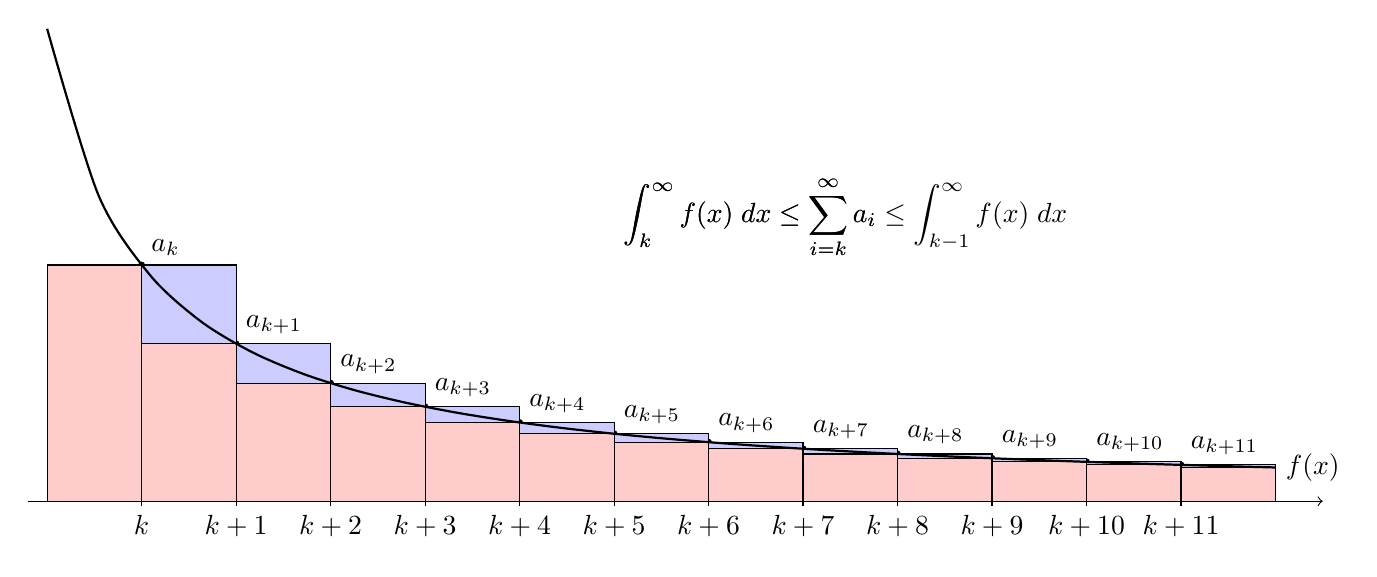
\begin{tikzpicture}[scale=1.2]
    \draw[white] (-1/3,-.5) rectangle (12.6,5);
    \draw[thin, ->] (-1.2,0) -- (12.5,0);
    \draw[thin] (0,0) +(0, .05) -- +(0, -.05)node[below]{$k$};
    \foreach \i in {1,2,...,11}{
        \draw[thin] (\i,0) +(0, .05) -- +(0, -.05)node[below]{$k + \i$};
    }
    \foreach \i in {0,1,2,...,11}{
        \pgfmathparse{5/(\i+2)}
        \draw[fill] (\i,\pgfmathresult) circle[radius=.03cm];
    }
    \node[above right] at (0,5/2) {$a_k$};
    \foreach \i in {1,2,...,11}{
        \pgfmathparse{5/(\i+2)}
        \node[above right] at (\i,\pgfmathresult) {$a_{k+\i}$};
    }
    \begin{scope}[svgfrag={2}{fade-out}]
        \begin{scope}[svgfrag={1}{fade-in}]
            \foreach \i in {0,1,2,...,11}{
                \pgfmathsetmacro{\y}{5/(\i+2)}
                \draw[fill=blue!20!white] (\i,0) rectangle +(1,\y);
            }
            \node[right] at (5,3) {$\displaystyle \int_{k}^\infty f(x)\;dx\le \sum_{i=k}^\infty a_i$};
        \end{scope}
    \end{scope}
    \begin{scope}[svgfrag={2}{fade-in}]
        \foreach \i in {0,1,2,...,12}{
            \pgfmathsetmacro{\y}{5/(\i+2)}
            \draw[fill=red!20!white] (\i,0) rectangle +(-1,\y);
        }
        \node[right] at (5,3) {$\displaystyle \int_{k}^\infty f(x)\;dx\le
        \sum_{i=k}^\infty a_i\le \int_{k-1}^\infty f(x)\;dx$};
    \end{scope}
    \draw[thick, domain=-1:12, smooth] plot (\x, {5/(\x + 2)})node[right]{$f(x)$};
\end{tikzpicture}
\end{document}
